\chapter{系统结果与评估}
\label{result}

本章节将会首先总结系统功能,然后简单对系统的性能、交互方式、虚实融合效果三部分进行最终结果的分析。

\section{系统功能汇总}
本系统实现了一个可以获得真实触感的增强现实应用。其中后端使用LibISR软件包,以及Kinect 2深度摄像头,实现对已知模型的物体进行追踪。

前端交互系统提供了注册、登陆、编著、交互四部分。编著系统提供了添加和移动物体、编辑物体、编辑实验场景、编辑实验流程和提示板、编辑已有实现等编著功能。交互系统通过和物体追踪系统进行网络交互,对单个创建的物体进行追踪、标定、显示。

综上所述,用户可以通过本应用,在手机或电脑端进行实验编辑,然后通过手机摄像头对场景中的对应真实物体进行追踪,并显示虚拟信息,实现有真实触感的增强现实应用。

\section{性能分析}

首先对物体追踪引擎仅进行追踪的时候的性能进行测试。物体追踪引擎运行环境为Intel Core i7 4790K处理器以及Nvidia GeForce GTX 980的显卡。

首先测试在仅进行单个物体追踪,没有网络传输的时候,服务器端的性能。其中为了准确仅计算了ISRCoreEngine中处理每一帧图像的时间,追踪结果如图\ref{fig:fps}所示,其中又左只有分别为开始追踪前、未找到追踪物体、追踪物体静止、追踪物体运动四种情况。帧率统计结果如图\ref{fig:fps}所示,其中横坐标为每一帧,纵坐标为对应的帧率。

\begin{figure}[!htp]
  \centering
  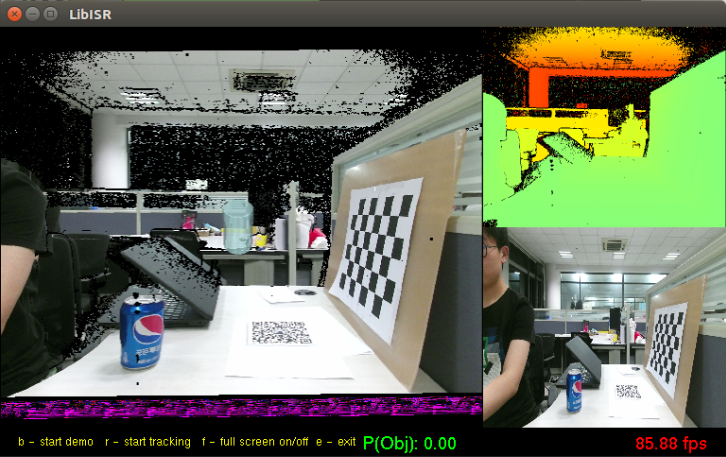
\includegraphics[width=3.3cm]{figure/beforeT.png}
  \hspace{0.1cm}
    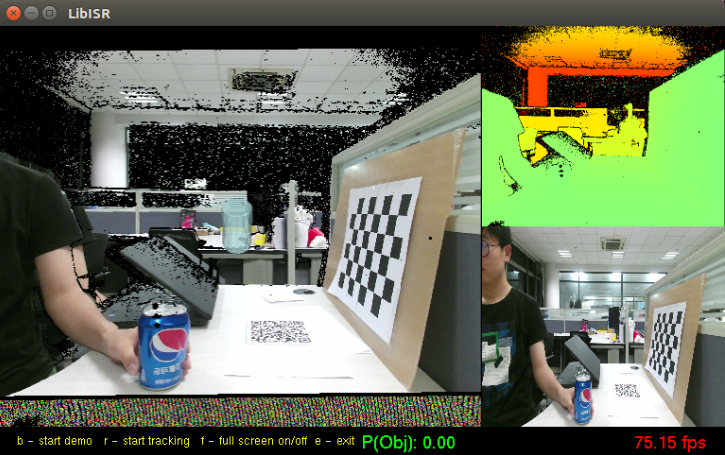
\includegraphics[width=3.3cm]{figure/noT.png}
  \hspace{0.1cm}
    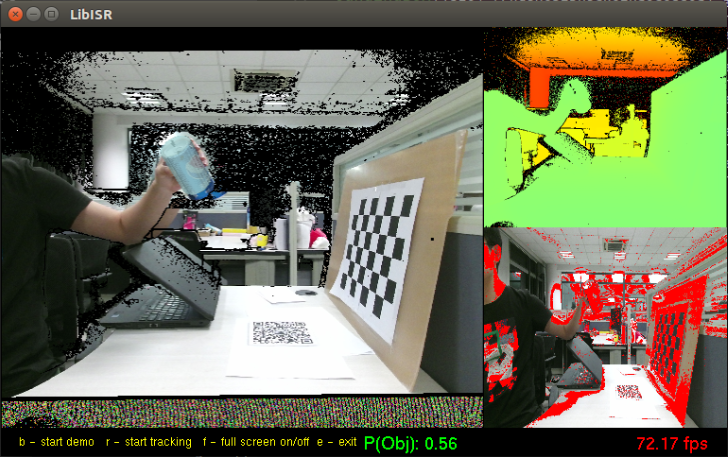
\includegraphics[width=3.3cm]{figure/staticT.png}
  \hspace{0.1cm}
  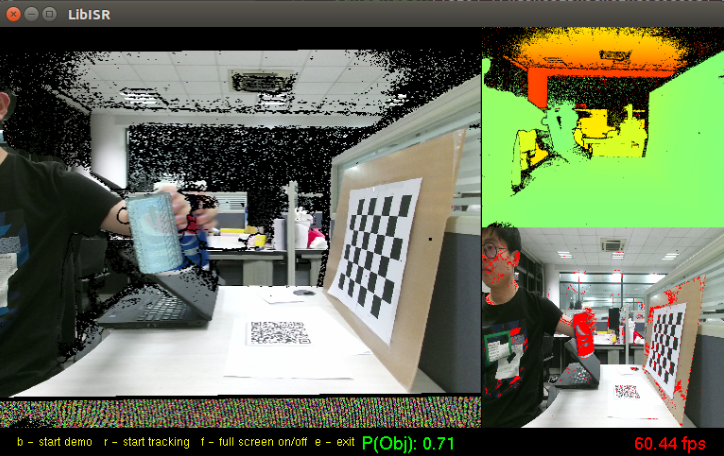
\includegraphics[width=3.3cm]{figure/movingT.png}
  \bicaption[物体追踪不同状态截图]
    {物体追踪不同状态截图}
    {The Screenshots of Tracing Object in Different Situations}
  \label{fig:SRR}
\end{figure}


\begin{figure}[!htp]
  \centering
  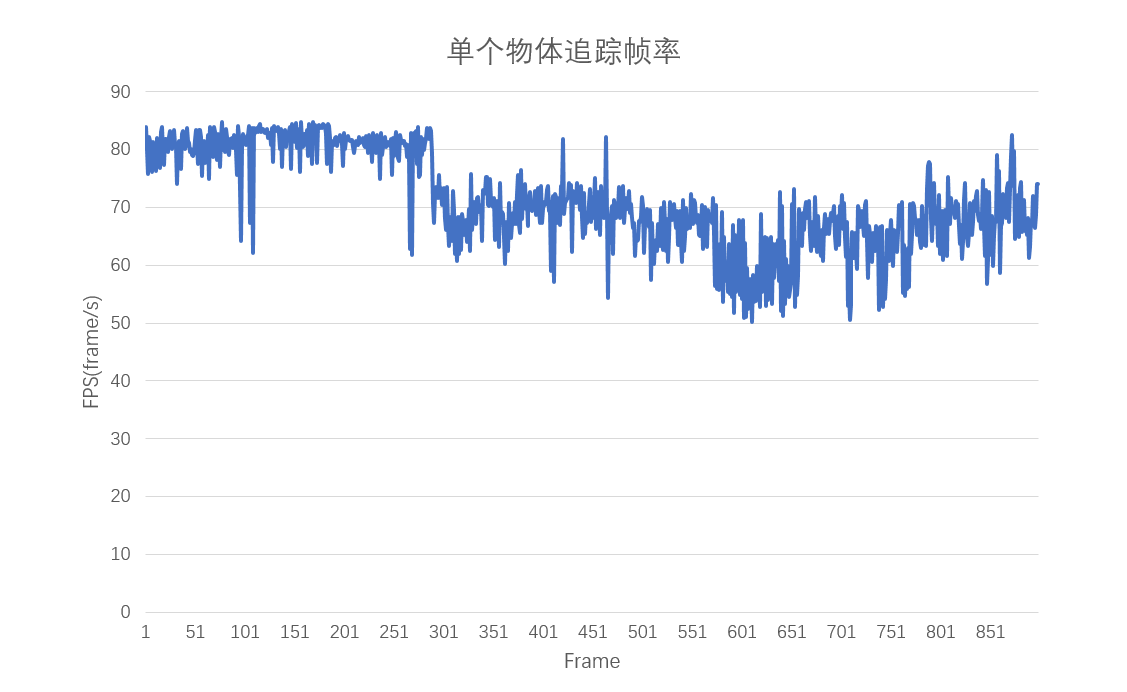
\includegraphics[width=10cm]{figure/fps.png}
  \bicaption[单个物体追踪帧-帧率折线图]
    {单个物体追踪帧-帧率折线图}
    {The Line Chart of Frame - Frame Per Second of Tracing Single Object }
 \label{fig:fps}
\end{figure}

从图中可以看出,在开始追踪之前,即仅测量从Kinect获取视频图像的性能,帧率约为80。从250帧左右开始追踪之后,帧率下降,当物体基本保持静止时或物体并没有被追踪到时,帧率约为70。当第550至650帧时,物体处于移动状态,帧率约为55帧。由此可见,帧率在追踪移动物体的时候性能消耗最大,但整体仍然满足60帧的性能需求。

之后在网络联通的情况下,在检测服务器上述速率的同时,检测客户端获取数据的速率,实际上也就是增强现实应用中物体运动姿态更新的频率。在程序中使用一个计数器,会在每次有数据接收的时候计数,然后每秒进行统计。客户端的运行环境为Intel Core i7 6500U处理器以及AMD Radeon R7 M370显卡。由于客户端和服务器在代码上保证了同步,因此该数据也代表了服务器的数据发送速率。经过测试,网络传输保持在每秒25次,这很大程度上是由于网络传输本身,以及实现的同步收发机制所限制的。此外,也利用Unity中的Coroutine进行每秒统计项目的帧数计算帧率,项目的帧率则被Unity保持在60。

最后,也检测了在移动端应用接受数据的传输速率。手机使用HiSilicon Kirin 970处理器。此时网络通讯速率仍然为每秒25次,项目帧率被Unity锁在30,但是实际上并不影响使用。

\section{编著系统交互分析}
系统在PC端和安卓手机端都进行了安装,两者都可以完成预期的工作。

在编著页面,使用手机的过程中,用户可以顺利完成点击、拖动等操作,实现全部预期需求,包括实验环境的修改,实验器具和药品的添加和编辑,实验流程的编辑、实验提示信息属性编辑等,其中手机端编辑药品属性和物质的量的菜单如图\ref{fig:mEdit}所示。所有的交互方式与PC端保持一致,只需要用手指触摸代替鼠标点击。此外,通过用户试用反馈来看,在物体的创建、编辑等部分用户可以很快上手,但是流程编辑的部分则有些复杂。

\begin{figure}[!htp]
  \centering
  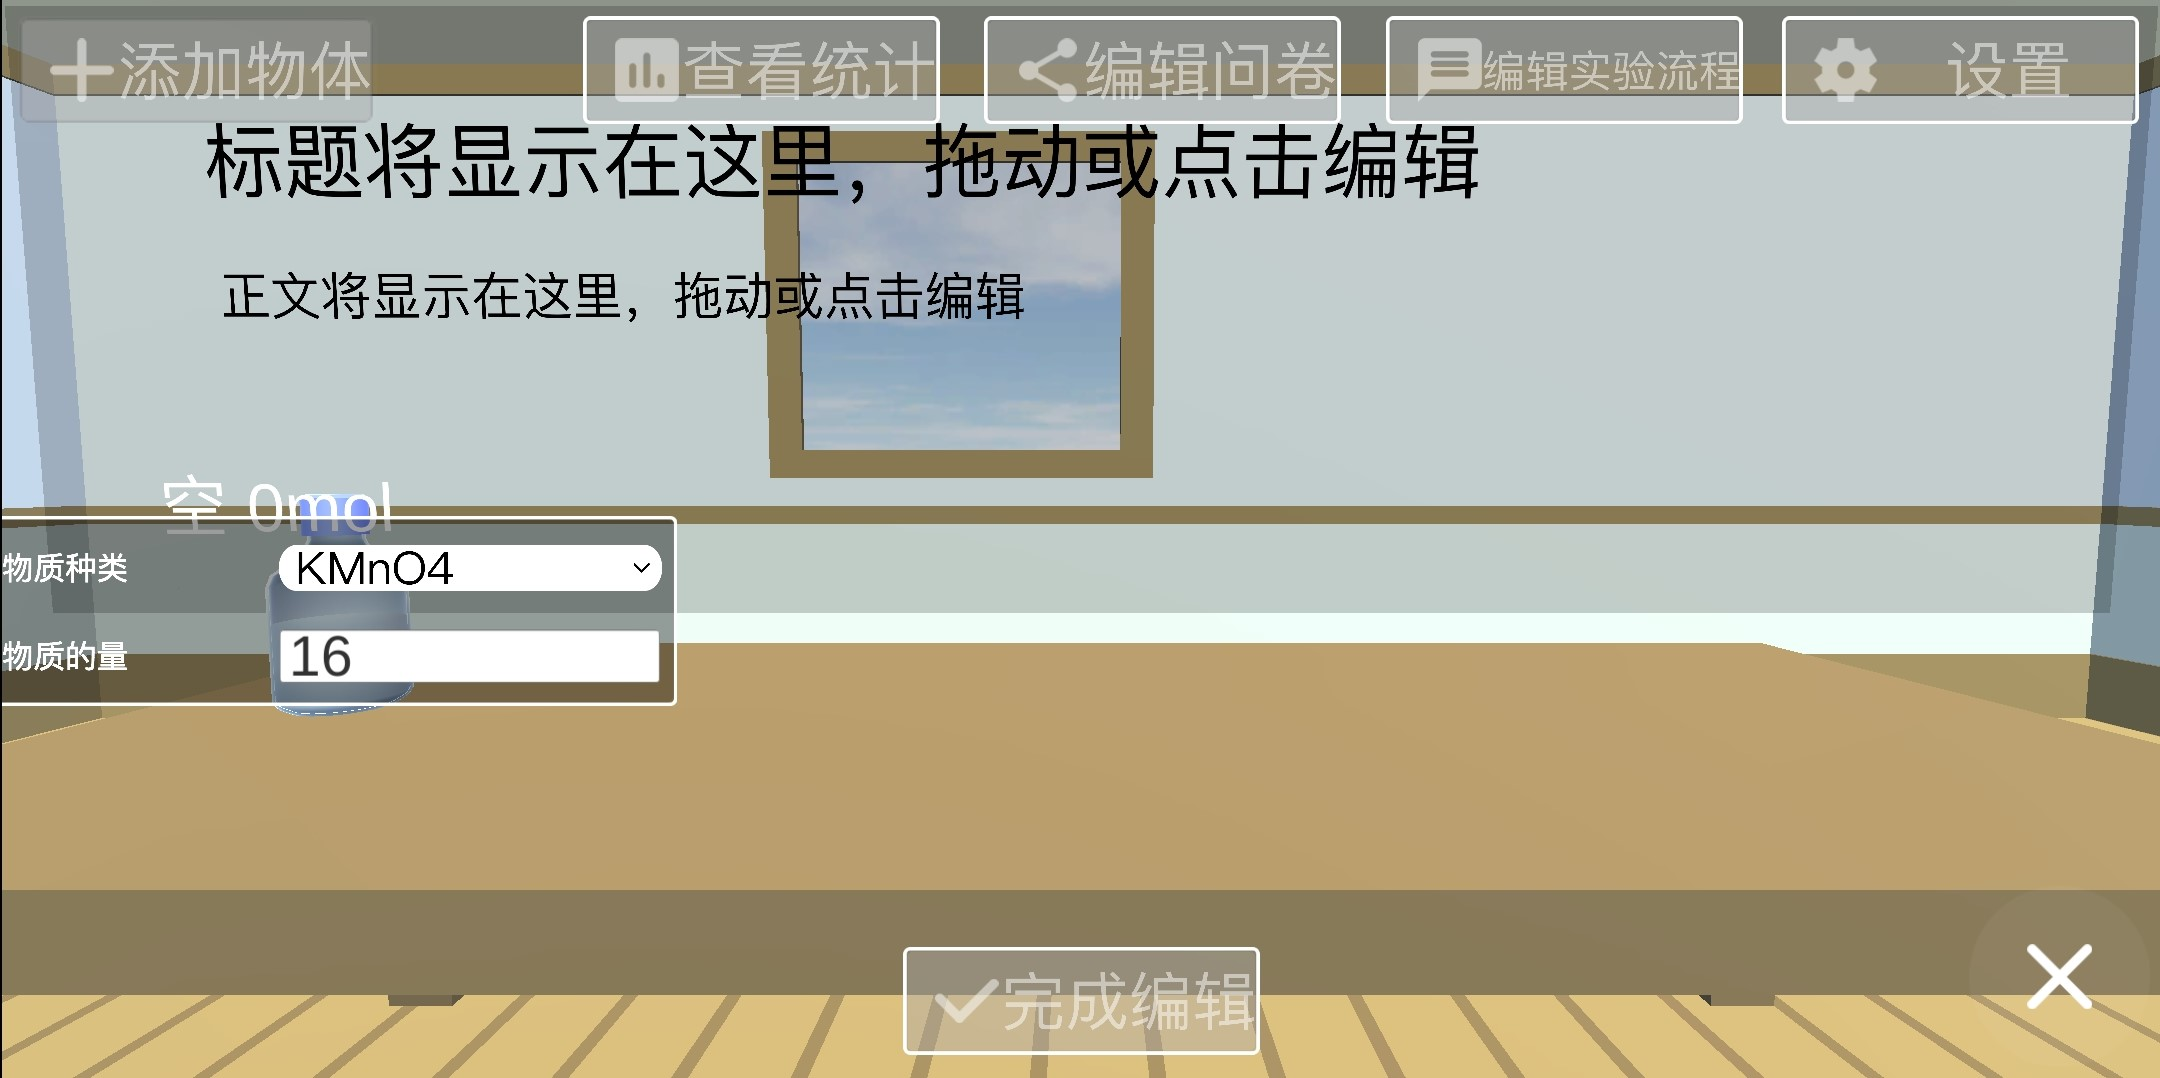
\includegraphics[width=12cm]{figure/mobileEdit.jpg}
  \bicaption[手机端编著系统截图]
    {手机端编著系统截图}
    {The Screenshot of Authoring System on Mobile Device}
 \label{fig:mEdit}
\end{figure}

\section{虚实融合效果分析}
在增强现实页面,用户可以通过手机向服务器发送指令,开始追踪,并且经过标定后,将虚拟物体与真实物体重合并且同步移动。在这个过程中,用户需要用手机拍摄到二维码,之后可以移动物体,观察手机中的虚拟图像。增强现实应用的用户界面与追踪效果如图\ref{fig:mAR}所示。

\begin{figure}[!htp]
  \centering
  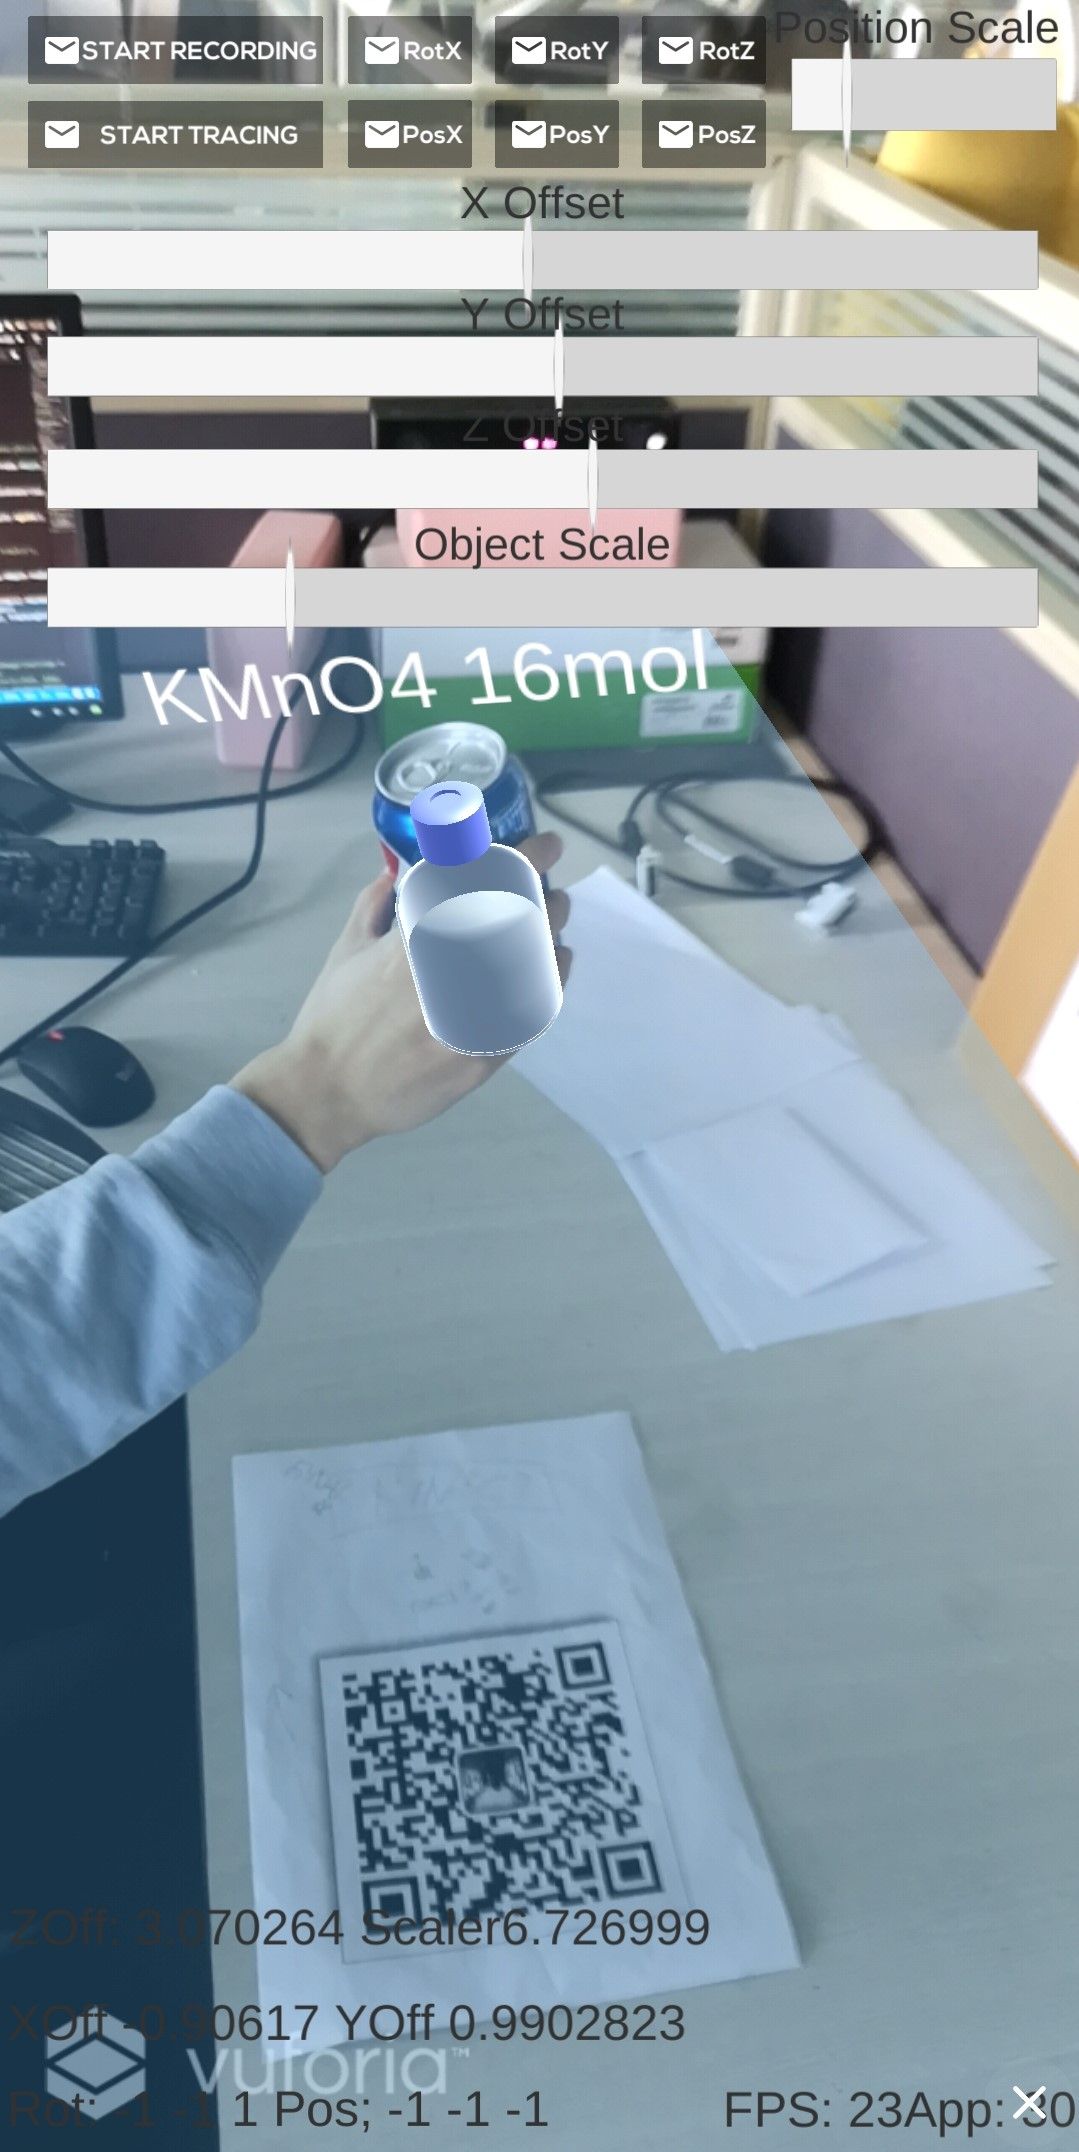
\includegraphics[width=6cm]{figure/mobileTrace.jpg}
  \bicaption[手机端增强现实场景截图]
    {手机端增强现实场景截图}
    {The Screenshot of AR System on Mobile Device}
 \label{fig:mAR}
\end{figure}

其中,图中的UI控件用与辅助用户进行标定。目前可以提前确定的数据都不再需要用户修改,用户只需要根据使用情景修改xyz三个方向上的偏移量就可以了。但是,由于Vuforia显示的虚拟物体是直接覆盖在摄像机图像上的,因此虚拟物体会覆盖在人手上,对于显示效果有一定的影响。

目前,虚拟物体实现与物体追踪服务器中得出的物体姿态数据保持完全一致。在比较精细的标定过程之后,也可以与真实物体进行比较好的融合。此外,虚拟物体也提供了一定的增强现实信息,包括虚拟的物体模型、虚拟物质及其含量提示等。

\section{本章小结}
本章对于物体追踪、网络传输等性能进行了一定的统计与分析,从软件层面和实际的应用体验来说,已经达到了预期要求。此外,也对于客户端的编著、增强现实交互的体验进行了一些分析,一定程度上满足了用户需求。